\documentclass[10pt]{article}
\usepackage{graphicx}
\graphicspath{{./images/}}
\begin{document}

%--------------------Title-------------------------
\begin{center}
\Huge{\textsc{Devendra Jadhav}}\bigskip
\end{center} 

%-------------To draw a Horizontal line------------------------
%\begin{tabular}{l}
%	\hline
%\end{tabular}

%--------------------SECTIONS-----------------------------------
%Section: Address \\
\begin{flushleft}
Bibwewadi, \\
Pune-37, Maharashtra \\
Contact: 8007097256 \\
Email ID: jadhav33devendra@gmail.com \\
LinkedIn ID: https://www.linkedin.com/in/devendra-jadhav-6a1a79100
\end{flushleft}

\begin{flushleft}
	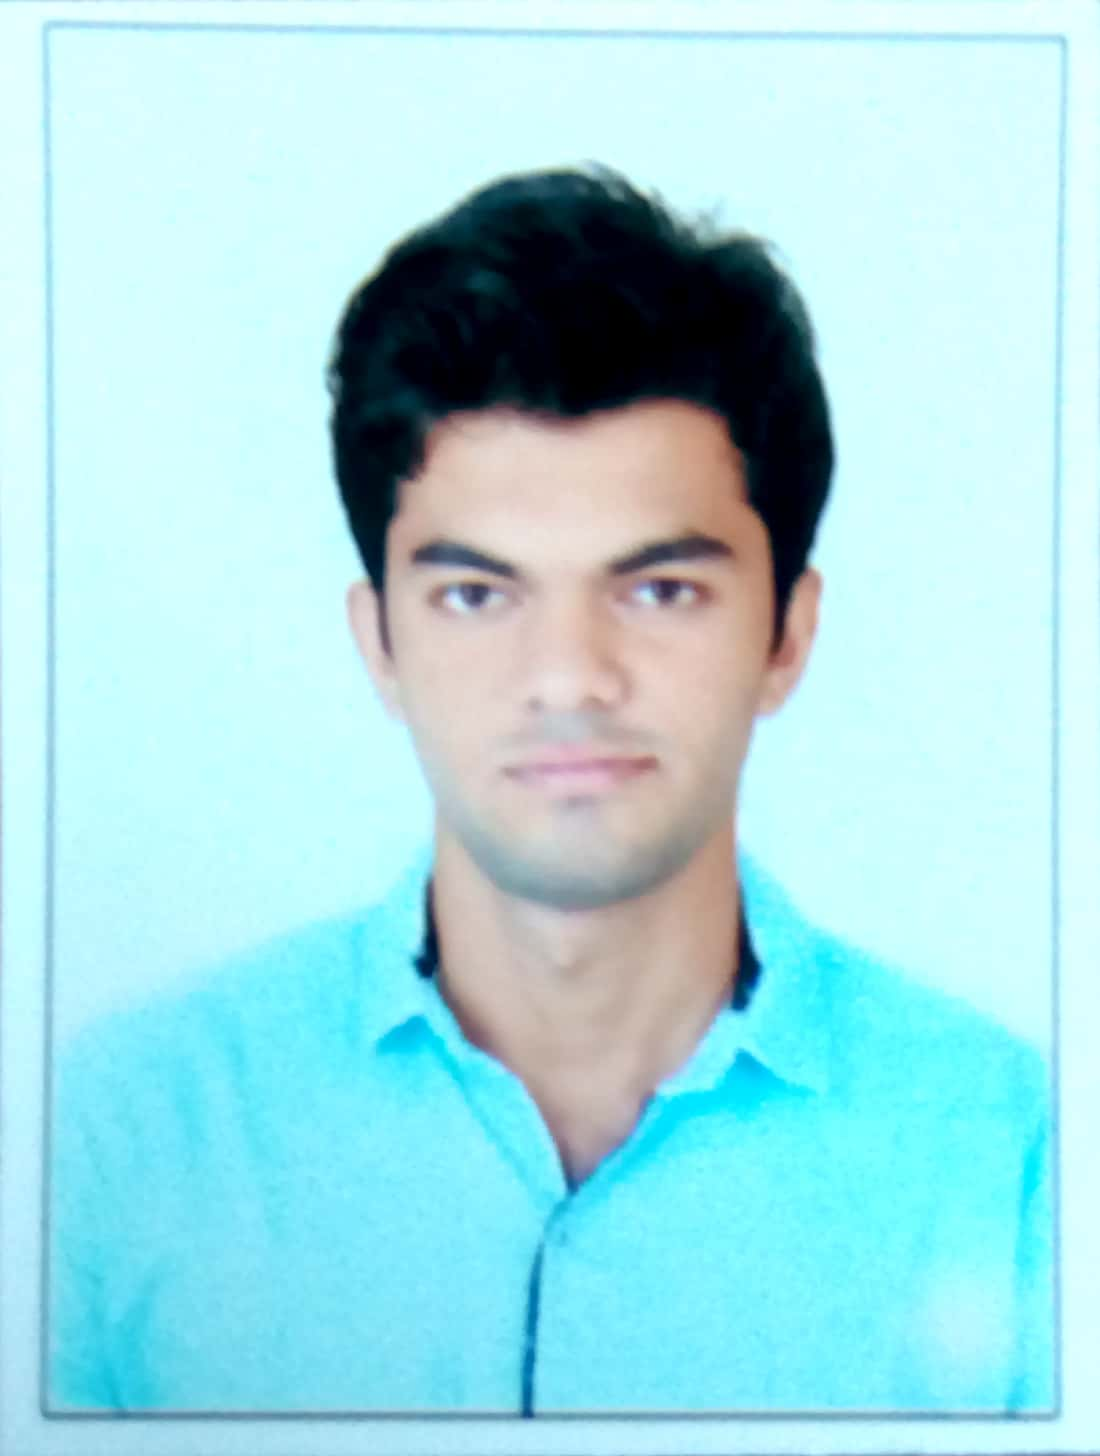
\includegraphics[scale=0.10]{dev.jpg}
\end{flushleft}


%Section: Career Objective
\begin{itemize}
	\bigskip
	\item  \LARGE{\textsc{Career Objective}} \\
	\small{A dynamic, team spirited and performance driven Mechanical engineering student aiming to gain knowledge and experience and apply my engineering skills to real world problems. Also to achieve and share my knowledge and gain information of new technology and implement it.} \\
	%\end{tabular}


%Section: Education
\bigskip
\item \begin{LARGE}
	\textsc{Education}
\end{LARGE} \\

\begin{tabular}{||c|c|c|c|c||}
	\hline
	
	Degree & College/School & University & Passing Year & Pass Percentage \\ 
	\hline
	TE Sem 5 & VIT, Pune & SPPU & Dec 2017 & 81.90\\\hline
	SE Sem 4 & VIT, Pune & SPPU & May 2017 & 82.537\\\hline
	SE Sem 3 & VIT, Pune & SPPU & Dec 2016 & 82.81\\\hline
	FE Sem 2 & VIT, Pune & SPPU & May 2016 & 83.629\\\hline
	FE Sem 1 & VIT, Pune & SPPU & Dec 2015 & 85.00\\\hline
	12\textsuperscript{th} & MSG College, Malegaon & - & June 2015 & 81.08 \\
	\hline10\textsuperscript{th} & KBH Vidyalaya, Malegaon & - & June 2013 & 90.91 \\\hline
\end{tabular}



%Section: Projects
\bigskip
\item \LARGE{\textsc{Projects}}
\begin{small}
	\begin{enumerate}
		\itemsep0em
		\item Automatic Vending Machine
		\item Bouncing Ball Game using 'simplecpp'
		\item Personal Carrier
		\item Vacuum Cleaner assisted with Floor Cleaner
		\item Simulation of Suspension System of a two wheeler 	
		\item 'Code for Designing Parking Facilities for Autonomous Vehicles using MATLAB'
		\item 'CFD Analysis of Fins' 
	\end{enumerate}


%Section: Training and Internship
\bigskip
\item \begin{LARGE}
	\textsc{Training and Internship}
\end{LARGE}\\

\begin{itemize}
	\itemsep0em
	\item[$\bullet$] Certification of 22 days Internship Program of Dassault Systemes on 3D-EXPERIENCE Essentials.
	\item[$\bullet$] Attended 3DSimulia Workshop
	\item[$\bullet$] Steam Engineering: Ongoing course sponsored by Forbes Marshall
\end{itemize}


%Section: Achivements
\bigskip
\item \begin{LARGE}
	\textsc{Achivements}
\end{LARGE}\\
\begin{enumerate}
	\itemsep0em
	\item Ranked 3rd in Spotter Snake theme in e-Yantra Robotics Competition National Finals held at IITB.
	\item Scored 295 marks out of 300 in 3DEXPERIENCE Associate - Mechanical Design Essentials at the level of Associate held at Dassault Systemes, Pune.
	\item Achieved 1st rank in ‘General Aptitude Exam’ in 11th standard.
\end{enumerate}


%Section: Technical Skillls
\bigskip
\item \begin{LARGE}
	\textsc{Technical Skillls}
\end{LARGE}\\

\begin{itemize}
	\itemsep0em
	\item[$\bullet$] Catia
	\item[$\bullet$] Autocad
	\item[$\bullet$] Solidworks
	\item[$\bullet$] Ansys
	\item[$\bullet$] MATLAB
	\item[$\bullet$] MS Excel
	\item[$\bullet$] 3DExperience
	\item[$\bullet$] 3DSimulia
	\item[$\bullet$] Fusion 360
\end{itemize}


%Section: Soft Skills
\bigskip
\item \begin{LARGE}
	\textsc{Soft Skills}
\end{LARGE}\\
\begin{enumerate}
	\itemsep0em
	\item Certification of Changing Gears Program sponsored by EATON in association with Confederation of Indian Industry (CII).
\end{enumerate}


%Section: Extra Curricular Activities
\bigskip
\item \begin{LARGE}
	\textsc{Extra Curricular Activities}
\end{LARGE}\\

\begin{itemize}
	\itemsep0em
	\item[$\bullet$] Worked in 'Aatmabodh-Our Knowledge for our Society' - A Social Event
	\item[$\bullet$] Attended Business workshop by EDC held in college.
	\item[$\bullet$] Represented school in Chess and Drawing competitions.
	\item[$\bullet$] Elementary and Intermediate exams of Drawing passed.
\end{itemize}


%Section: Co-Curricular Activities
\bigskip
\item \begin{LARGE}
	\textsc{Co-Curricular Activities}
\end{LARGE}\\
\begin{enumerate}
	\itemsep0em
	\item 'Spotter Snake' Robot in e-Yantra Robotics Competition.
	\item Member of Team Veloce Racing, participating in racing competitions like SAESUPRA.
\end{enumerate}


%Section: Professional Skills
\bigskip
\item \begin{LARGE}
	\textsc{Professional Skills}
\end{LARGE} \\

\begin{itemize}
	\itemsep0em
	\item[$\bullet$] Good Team Player
	\item[$\bullet$] Willingness to learn and progress
\end{itemize}


%Section: Hobbies
\bigskip
\item \begin{LARGE}
	\textsc{Hobbies}
\end{LARGE}\\
\begin{enumerate}
	\itemsep0em
	\item Music 
	\item Solving Aptitude problems
	\item Trekking and Travelling
\end{enumerate}


%Section: Languages
\bigskip
\item \begin{LARGE}
	\textsc{Languages}
\end{LARGE} \\

\begin{itemize}
	\itemsep0em
	\item[$\bullet$] German(Basic)
	\item[$\bullet$] French(Basic)
	\item[$\bullet$] English
	\item[$\bullet$] Hindi
	\item[$\bullet$] Marathi
\end{itemize}



\end{small}
\end{itemize}
\end{document}